% !TeX spellcheck = en_US
\documentclass[letterpaper,12pt,twoside]{report}
\usepackage{fancyhdr}
\usepackage{fullpage}
\usepackage{tikz}
\usepackage{amsmath}

\begin{document}
	\pagestyle{fancy}
	\fancyhf{}
	\fancyhead[L]{Day 19}
	\fancyhead[R]{\textit{The Calendar Project}}
	\fancyfoot[L]{Citations Involved: none}
	
	% Problem
	\paragraph{Problem}
	\begin{quote}
		\textsf{The volume of a rectangular prism
			is 864 $\text{cm}^\text{3}$. Two if its faces have areas of
			72 $\text{cm}^\text{2}$
			and 96 $\text{cm}^\text{2}$. Find the length of a
			diagonal that connects a pair of opposite
			vertices of the prism.}
	\end{quote}
	
	% Graphics
	\begin{center}
		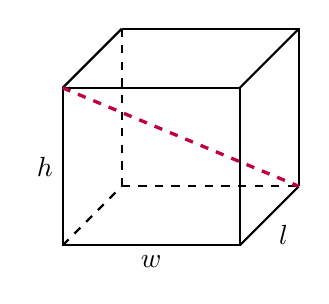
\begin{tikzpicture}[scale=0.25]
		\draw[thick] (0,0) -- (9,0) -- (9,8) -- (0,8) -- cycle;
		\draw[thick][dashed] (0,0) -- (3,3);
		\draw[thick] (9,0) -- (12,3);
		\draw[thick] (9,8) -- (12,11);
		\draw[thick] (0,8) -- (3,11);
		\draw[thick] (3,11) -- (12,11) -- (12,3);
		\draw[thick][dashed] (3,3) -- (3,11);
		\draw[thick][dashed] (3,3) -- (12,3);
		
		\node[below] at (4.5,0) {$w$};
		\node[left] at (0,4) {$h$};
		\node[below right] at (10.5,1.5) {$l$};
		
		\draw[very thick][dashed][purple] (0,8) -- (12,3);
		\end{tikzpicture}
	\end{center}
	
	% Reasoning
	\paragraph{Reasoning}
	\begin{quotation}
		
		The formula for the volume of a rectangular prism is $whl$ where $w$ is its width, $h$ is its height, and $l$ is its length (2). Given that the volume of the rectangular prism is 864 $\text{cm}^3$, $whl=864$. Let the two faces whose areas have been specified be $wh$ and $hl$; as such, $wh=72$ and $hl=96$. The variables are solved according to this system of equations as follows:
		
		\begin{center}
			\begin{tabular}{l | l}
				$72l=864$ & Substitution Property from $whl=864$ and $wh=72$ \\
				$l=12$ & Simplify \\
				\hline
				$12h=96$ & Substitution Property from $hl=96$ \\
				$h=8$ & Simplify \\
				\hline
				$8w=72$ & Substitution Property from $wh=72$ \\
				$w=9$ & Simplify
			\end{tabular}
		\end{center}
		
		The formula for the diagonal connecting a pair of opposite vertices in a rectangular prism is $\sqrt{w^2+h^2+l^2}$ (1); this evaluates to $\sqrt{9^2+8^2+12^2}=\sqrt{81+64+144}=\sqrt{289}=\boxed{17 \text{ cm}}$.
	\end{quotation}
	
	\paragraph{External References}
	
	\begin{enumerate}
		\item Textbook Ch. 10, Pg. 672: Distance and Midpoint Formulas in Three Dimensions
		\item Textbook Ch. 10, Pg. 697: Volume of a Prism
	\end{enumerate}
	
\end{document}